\chapter{Th\'eorie des circuits AC} \label{subsec:ac_circuit_theory}

\section{Introduction au courant alternatif} \label{subsec:intro_ac}
Le \emph{courant alternatif} (souvent not\'e \textbf{AC} pour \emph{Alternating Current}) est un type de courant \'electrique dont l’intensit\'e et la direction varient p\'eriodiquement au cours du temps. Contrairement au courant continu (DC), où les \'electrons circulent toujours dans le même sens, le courant alternatif change de sens à intervalles r\'eguliers, g\'en\'eralement selon une forme sinuso\"idale.\par
Il est g\'en\'eralement repr\'esent\'e pas une onde sinuso\"idale~:
\[
    u(t) = U_{max} \cdot \sin(\omega t + \phi)
\]
o\`u :
\begin{itemize}
    \item $u(t)$ est la tension instantan\'ee en fonction du temps $t$,
    \item $U_{max}$ est l'amplitude maximale de la tension,
    \item $\omega$ est la pulsation angulaire (en radians par seconde), reli\'ee à la fr\'equence $f$ par la relation $\omega = 2\pi f$,
    \item $\phi$ est la phase initiale (en radians), qui d\'etermine le d\'ecalage de l'onde par rapport au temps $t = 0$.
\end{itemize}

\subsection{La phase}
La \emph{phase} d'une onde sinuso\"idale d\'efinit son \emph{d\'ecalage temporel} par rapport à une r\'ef\'erence. Elle est exprim\'ee en radians (ou en degr\'es) et indique \`a quel point l'onde commence dans son cycle au temps $t = 0$.\par

\begin{figure}[h!]
    \newcounter{angle}
    \setcounter{angle}{220}
    \begin{tikzpicture}
    \draw[thick,-stealth,black] (-3,0)--(4,0) coordinate (A) node[below] {$x$};
    \draw[thick,-stealth,black] (0,-3)--(0,3) node[left] {$y$}; % y axis
    \draw[black,thin] (0,0) circle (2.5cm);
    \node[black,below] at (2.7,0) {1};
    \node[black,above] at (0.2,-3.2) {1};
    \draw (1,0) arc (0:\theangle:1) node at ($(\theangle/2:0.7)$) {$\phi$};
    \draw[dashed, blue] (\theangle:2.5cm) -- (\theangle:2.5cm |- 0,0) node[sloped, rotate=180, yshift=8pt, midway] {$\sin \phi$}; % vertical line
    \draw[ultra thick,red,rotate=\theangle] (0,0) -- (2.5,0) coordinate (B);
    \foreach \x in {0,30,...,360} {\filldraw[black] (\x:2.5cm) circle(1pt);};
    \foreach \x/\xtext in {
            30/\frac{\pi}{6},
            60/\frac{\pi}{3},
            120/\frac{2\pi}{3},
            150/\frac{5\pi}{6},
            210/\frac{7\pi}{6},
            240/\frac{4\pi}{3},
            300/\frac{5\pi}{3},
            330/\frac{11\pi}{6}
            }
        \draw (\x:2.8cm) node {\tiny $\xtext$};
    \foreach \x/\xtext in {
            90/\frac{\pi}{2}}
            \draw (\x:2.7cm) node[xshift=4pt] {\tiny $\xtext$};
    \foreach \x/\xtext in {
            270/\frac{3\pi}{2}}
            \draw (\x:2.7cm) node[xshift=-5pt] {\tiny $\xtext$};
    \foreach \x/\xtext in {
            180/\pi,
            360/2\pi}
            \draw (\x:2.7cm) node[yshift=4pt] {\tiny $\xtext$};

    \begin{scope}
    \begin{axis}[
        thick,
        y=2.5cm,
        axis lines=center,
        xmin=0, xmax=360,
        ymin=-1, ymax=1,
        anchor=origin, at=(A),
        xshift=3ex,
        enlarge y limits,
        enlarge x limits=upper,
        samples=90,
        xtick={0,30,...,360},
    xticklabels={0,
        $\frac{\pi}{6}$,
        $\frac{\pi}{3}$,
        $\frac{\pi}{2}$,
        $\frac{2\pi}{3}$,
        $\frac{5\pi}{6}$,
        $\pi$,
        $\frac{7\pi}{6}$,
        $\frac{4\pi}{3}$,
        $\frac{3\pi}{2}$,
        $\frac{5\pi}{3}$,
        $\frac{11\pi}{6}$,
        $2\pi$
        },
        tick label style={font=\tiny},
        ]
        \addplot[domain=0:\theangle,ultra thick, no markers,blue] {sin(x)} coordinate (C);
        \addplot[domain=\theangle-1:\theangle,ultra thick, no markers,blue] {sin(x)-sin(x)} coordinate (K);
    \end{axis}
    \draw [dashed,red, thick] (B) -- (C);
    \draw [dashed,blue, thick] (C) -- (K);
    \end{scope}
    \tkzDrawPoints(B);
    \end{tikzpicture}
    \label{fig:phase}
    \caption{Repr\'esentation de la phase $\phi$ d'une onde sinuso\"idale.}
\end{figure}

\subsection{Valeur efficace (RMS)}
La valeur efficace (ou RMS, \emph{Root Mean Square}) d'une tension ou d'un courant alternatif est une mesure de la valeur moyenne de la puissance dissip\'ee par le courant.
Pour une onde sinuso\"idale, la valeur efficace de tension et de courant sont donn\'ees par~:
\[
U_{\text{eff}} = \frac{U_{\text{max}}}{\sqrt{2}}, \quad I_{\text{eff}} = \frac{I_{\text{max}}}{\sqrt{2}}
\]
\begin{Note}{\textbf{D'où vient le $\sqrt{2}$ ?}}\\
La formule g\'en\'erale de la valeur efficace est~:
\[
U_{\text{eff}} = \sqrt{\frac{1}{T_2 - T_1} \int_{T_1}^{T_2} [u(t)]^2 \, dt}
\]
avec \( u(t) = U_{\text{max}}\sin(\omega t) \). On obtient alors~:
\[
U_{\text{eff}} = U_{\text{max}} \sqrt{\frac{1}{T_2 - T_1} \int_{T_1}^{T_2} \sin^2(\omega t)\, dt}
\]
En utilisant l'identit\'e trigonom\'etrique $\sin^2(x) = \frac{1 - \cos(2x)}{2}$, on peut \'ecrire~:
\[
\int_{T_1}^{T_2} \sin^2(\omega t)\, dt = \frac{1}{2}(T_2 - T_1)
\]
puisque l’int\'egrale du terme $\cos(2\omega t)$ sur une p\'eriode compl\`ete est nulle.
Ainsi :
\[
U_{\text{eff}} = U_{\text{max}} \sqrt{\frac{1}{T_2 - T_1} \cdot \frac{T_2 - T_1}{2}} = \frac{U_{\text{max}}}{\sqrt{2}}
\]
\end{Note}
Pour une onde carr\'ee, la valeur efficace est \'egale à l'amplitude maximale~:
\[U_{\text{eff}} = U_{\text{max}}, \quad I_{\text{eff}} = I_{\text{max}}\]
Pour une onde triangulaire, la valeur efficace est donn\'ee par~:
\[U_{\text{eff}} = \frac{U_{\text{max}}}{\sqrt{3}}, \quad I_{\text{eff}} = \frac{I_{\text{max}}}{\sqrt{3}}\]


\subsection{Puissance en AC}
La puissance dans un circuit en courant alternatif d\'epend non seulement de la tension et du courant, mais aussi du d\'ephasage $\phi$ entre eux.
La tension et le courant peuvent être exprim\'es sous forme sinuso\"idale :
\[
u(t) = U_{\text{max}} \sin(\omega t), \quad i(t) = I_{\text{max}} \sin(\omega t - \phi)
\]
La puissance instantan\'ee vaut alors :
\[
p(t) = u(t) \cdot i(t) = U_{\text{max}} I_{\text{max}} \sin(\omega t)\sin(\omega t - \phi)
\]
En utilisant l'identit\'e trigonom\'etrique $\sin A \sin B = \tfrac{1}{2}[\cos(A - B) - \cos(A + B)]$, on obtient :
\[
p(t) = \frac{U_{\text{max}} I_{\text{max}}}{2} [\cos(\phi) - \cos(2\omega t - \phi)]
\]
La puissance instantan\'ee est donc constitu\'ee d’un terme constant et d’un terme variable à la fr\'equence double.

\begin{Note}{\textbf{Puissance moyenne (active)}}\\
Le terme oscillant $\cos(2\omega t - \phi)$ a une moyenne nulle sur une p\'eriode complète.
La puissance moyenne (ou puissance active) est donc :
\[
P = \frac{U_{\text{max}} I_{\text{max}}}{2} \cos(\phi)
\]
En exprimant les grandeurs en valeurs efficaces :
\[
U_{\text{eff}} = \frac{U_{\text{max}}}{\sqrt{2}}, \quad I_{\text{eff}} = \frac{I_{\text{max}}}{\sqrt{2}}
\]
on obtient la relation fondamentale :
\[
\boxed{P = U_{\text{eff}} \cdot I_{\text{eff}} \cdot \cos(\phi)}
\]
où :
\begin{itemize}
    \item $P$ est la puissance active (en watts, W),
    \item $U_{\text{eff}}$ est la tension efficace (en volts, V),
    \item $I_{\text{eff}}$ est le courant efficace (en ampères, A),
    \item $\phi$ est le d\'ephasage entre la tension et le courant.
\end{itemize}
\end{Note}

\subsubsection*{Les diff\'erentes puissances en r\'egime alternatif}
On distingue trois formes de puissance :
\begin{itemize}
    \item \textbf{Puissance apparente}~:
    \[
    S = U_{\text{eff}} I_{\text{eff}} \quad [\text{VA}]
    \]
    Elle repr\'esente la puissance totale fournie au circuit.

    \item \textbf{Puissance active}~:
    \[
    P = U_{\text{eff}} I_{\text{eff}} \cos(\phi) \quad [\text{W}]
    \]
    Elle correspond à la puissance r\'eellement consomm\'ee ou convertie en travail ou chaleur.

    \item \textbf{Puissance r\'eactive}~:
    \[
    Q = U_{\text{eff}} I_{\text{eff}} \sin(\phi) \quad [\text{var}]
    \]
    Elle repr\'esente l’\'energie \'echang\'ee p\'eriodiquement entre les champs \'electrique et magn\'etique des composants r\'eactifs (bobines et condensateurs).
\end{itemize}

Ces trois puissances sont li\'ees par la relation :
\[
S^2 = P^2 + Q^2
\]
et peuvent être repr\'esent\'ees sous forme d’un \textbf{triangle des puissances}.
Le \emph{facteur de puissance}, not\'e $\cos(\phi)$, indique la part de puissance r\'eellement utilis\'ee par le circuit :
\[
\text{Facteur de puissance} = \frac{P}{S} = \cos(\phi)
\]
Un facteur de puissance proche de \(1\) signifie un usage efficace de l’\'energie \'electrique, tandis qu’un facteur faible traduit une forte composante r\'eactive.
\begin{figure}[h!]
\centering
\begin{tikzpicture}
  \begin{axis}[
    axis lines=middle,
    xlabel={$P$ (W)},
    ylabel={$Q$ (var)},
    xmin=0, xmax=3.8,
    ymin=0, ymax=2.8,
    grid=both,
    width=9cm, height=6cm,
    axis equal image,
    xtick=\empty, ytick=\empty,
    enlargelimits=false,
    axis line style={thick,-latex},
    every axis y label/.style={
        at={(ticklabel cs:0.5)},rotate=90,anchor=near ticklabel,
    },
    every axis x label/.style={
        at={(ticklabel cs:0.5)},anchor=near ticklabel,
    },
  ]
  \coordinate (O) at (axis cs:0,0);
  \coordinate (A) at (axis cs:3,0);   % P
  \coordinate (B) at (axis cs:3,2);   % Q
  \draw[thick, blue] (O) -- node[below, yshift=-2pt] {$P$} (A);
  \draw[thick, red] (A) -- node[right, xshift=2pt] {$Q$} (B);
  \draw[thick, black] (O) -- node[above, rotate=35] {$S=\sqrt{P^2+Q^2}$} (B);
  \draw pic["$\phi$", draw=black, angle radius=8mm, angle eccentricity=1.2] {angle = A--O--B};
  \node at (axis cs:1.5,0.5) {\small $\cos\phi = \dfrac{P}{S}$};
  \end{axis}
\end{tikzpicture}
\caption{Triangle des puissances en r\'egime alternatif : relation entre $P$, $Q$ et $S$.}
\label{fig:triangle_puissances}
\end{figure}

\section{Circuits RLC} \label{subsec:rlc_circuits}
\subsection{Comportement des composants en AC}
\subsubsection{Résistance (R)}
Une r\'esistance (not\'ee \(R\)) dans un circuit en courant alternatif se comporte de la m\^eme mani\`ere qu'en courant continu. Elle ob\'eit à la loi d'Ohm. La tension et le courant sont en phase, c'est-à-dire qu'ils atteignent leurs valeurs maximales et minimales en m\^eme temps. La relation entre la tension et le courant est donn\'ee par~:
\[u(t) = R \cdot i(t)\]
Son imp\'edance est purement r\'eelle et vaut \(Z = R\).

\subsubsection{Inductance (L)}
Une inductance (not\'ee \(L\)) est un composant qui stocke de l'\'energie dans un champ magn\'etique lorsqu'un courant le traverse. En courant alternatif, l'inductance oppose une r\'esistance au changement de courant, ce qui provoque un d\'ecalage de phase entre la tension et le courant. La tension à travers une inductance est donn\'ee par~:
\[u(t) = L \frac{di(t)}{dt}\]
Dans un circuit en AC, la tension à travers une inductance est en avance de \(\frac{\pi}{2}\) (90 degr\'es) par rapport au courant.
L'imp\'edance d'une inductance est donn\'ee par~:
\[Z_L = j\omega L\]
o\`u \(\omega = 2\pi f\) est la pulsation angulaire. L'imp\'edance est purement imaginaire et positive, indiquant une r\'eactance inductive.
\begin{figure}[h!]
	\centering
	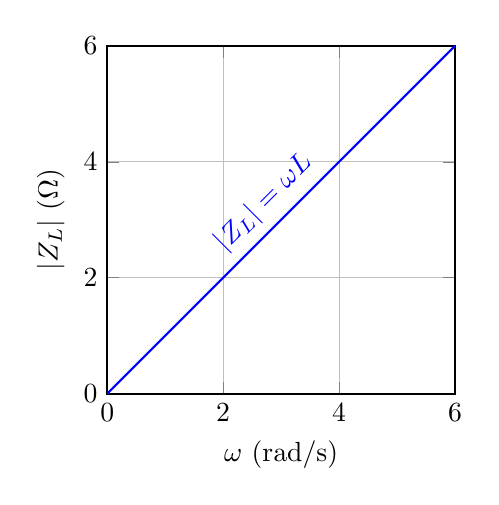
\begin{tikzpicture}
	    \begin{axis}[
            xlabel={$\omega$ (rad/s)},
            ylabel={$|Z_L|$ ($\Omega$)},
            xmin=0, xmax=6,
            ymin=0, ymax=6,
            grid=both,
            width=10cm, height=6cm,
            axis equal image,
            enlargelimits=false,
            axis line style={thick,-latex},
            every axis y label/.style={
                at={(ticklabel cs:0.5)},rotate=90,anchor=near ticklabel,
            },
            every axis x label/.style={
                at={(ticklabel cs:0.5)},anchor=near ticklabel,
            },
        ]
        \addplot[domain=0:6, thick, blue] {x} node[pos=0.5, above, rotate=45] {$|Z_L| = \omega L$};
        \end{axis}
    \end{tikzpicture}
    \caption{Imp\'edance d'une inductance en fonction de la pulsation angulaire $\omega$.}
    \label{fig:impedance_inductance}
\end{figure}

\subsubsection{Capacit\'e (C)}
Un condensateur (not\'e \(C\)) est un composant qui stocke de l'\'energie dans un champ \'electrique. En courant alternatif, le condensateur permet au courant de passer plus facilement à mesure que la fr\'equence augmente, ce qui provoque un d\'ecalage de phase entre la tension et le courant. La relation entre la tension et le courant dans un condensateur est donn\'ee par~:
\[i(t) = C \frac{du(t)}{dt}\]
Dans un circuit en AC, le courant à travers un condensateur est en avance de \(\frac{\pi}{2}\) (90 degr\'es) par rapport à la tension.
L'imp\'edance d'un condensateur est donn\'ee par~:
\[Z_C = \frac{1}{j\omega C} = -j\frac{1}{\omega C}\]
L'imp\'edance est purement imaginaire et n\'egative, indiquant une r\'eactance capacitive.
\begin{figure}[h!]
    \centering
    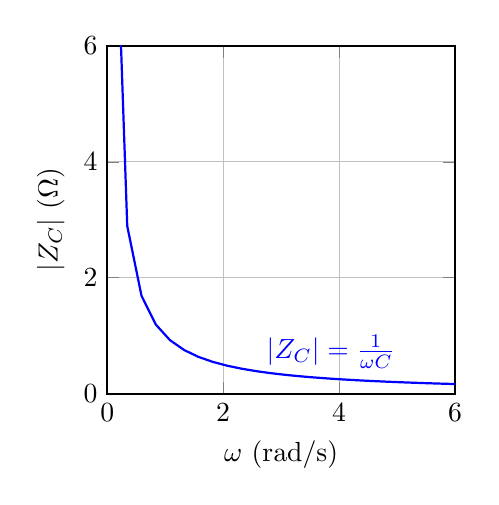
\begin{tikzpicture}
        \begin{axis}[
            xlabel={$\omega$ (rad/s)},
            ylabel={$|Z_C|$ ($\Omega$)},
            xmin=0, xmax=6,
            ymin=0, ymax=6,
            grid=both,
            width=10cm, height=6cm,
            axis equal image,
            enlargelimits=false,
            axis line style={thick,-latex},
            every axis y label/.style={
                at={(ticklabel cs:0.5)},rotate=90,anchor=near ticklabel,
            },
            every axis x label/.style={
                at={(ticklabel cs:0.5)},anchor=near ticklabel,
            },
        ]
        \addplot[domain=0.1:6, thick, blue] {1/x} node[pos=0.85, above] {$|Z_C| = \frac{1}{\omega C}$};
        \end{axis}
    \end{tikzpicture}
    \caption{Imp\'edance d'un condensateur en fonction de la pulsation angulaire $\omega$.}
    \label{fig:impedance_condensateur}
\end{figure}


\section{Filtres et r\'eponse en fr\'equence} \label{subsec:filters}
\section{Transformateurs et \'electromagn\'etisme} \label{subsec:transformers}
\section{Alimentations et \'electronique de puissance} \label{subsec:power_supplies}
